%------------------ Data, time regime, area ---------------------------
\section{Data \& area}

In this tab the user can set the contact point as well as other important points of the indentation process, mechanical properties of the tip and sample, indenter noise and define the area function.
After successfully loading a file, the software creates the force-distance diagram from the data, and attempts to automatically detect the loading, hold and unloading parts of the data.

\begin{figure}[ht]
  \centering
  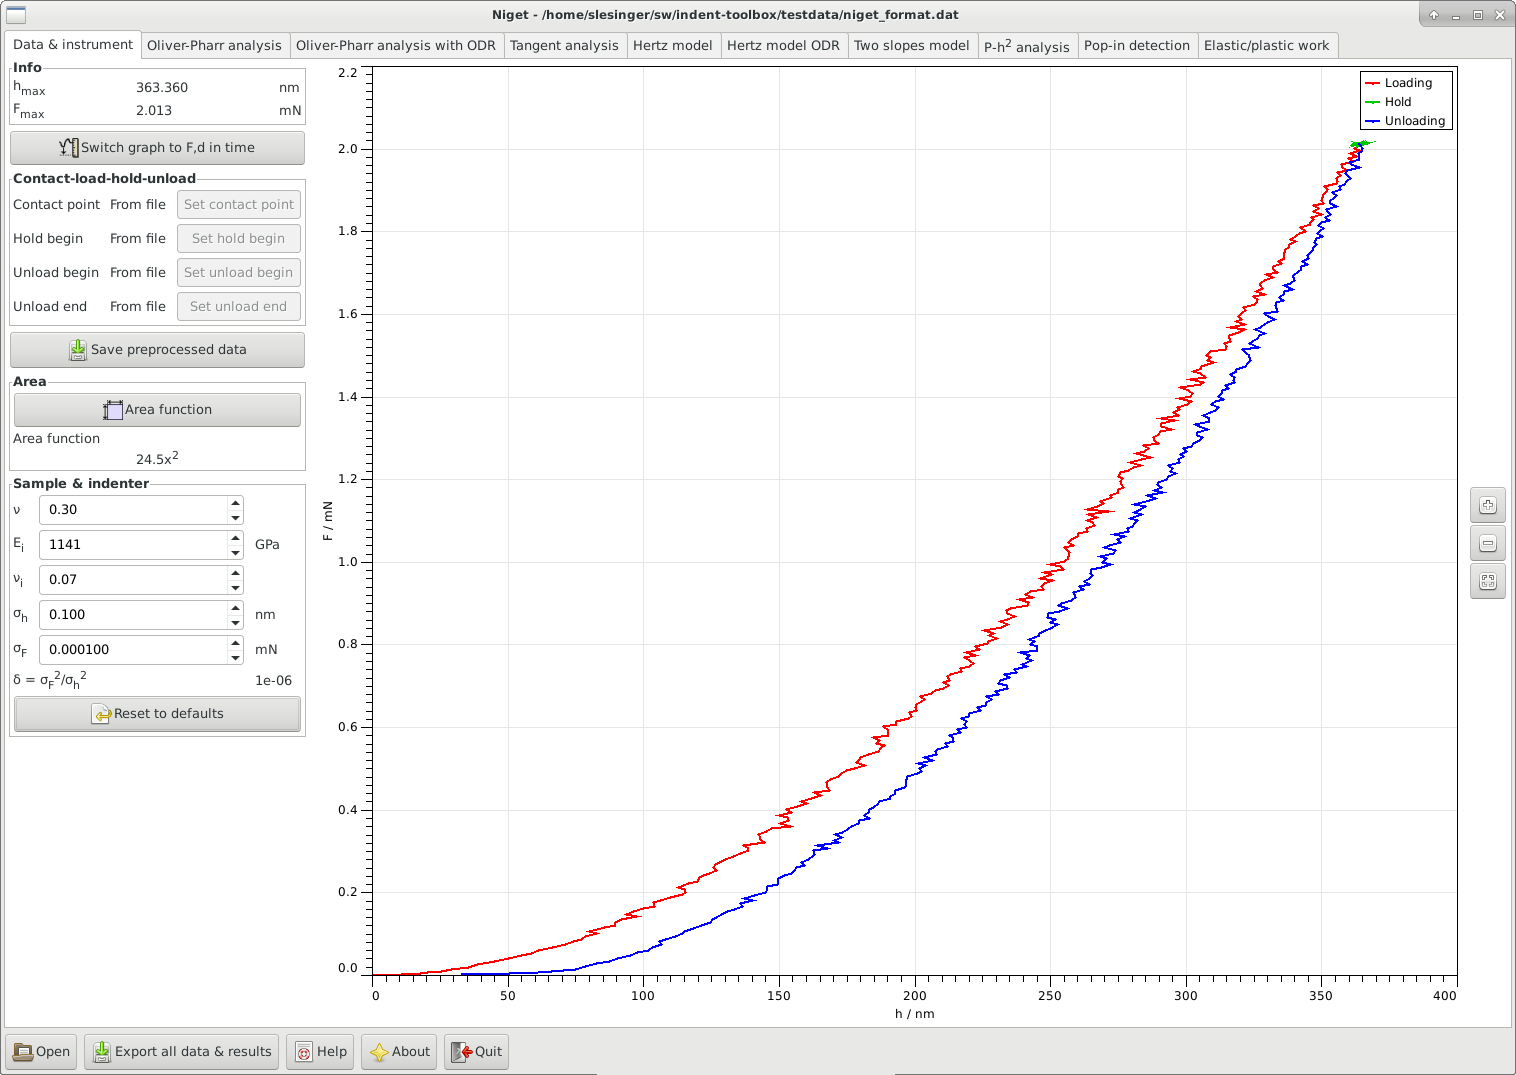
\includegraphics[width=\textwidth]{images/screen-fd}
  \caption{Force-distance diagram after automatic split}
\end{figure}

\begin{figure}[ht]
  \centering
  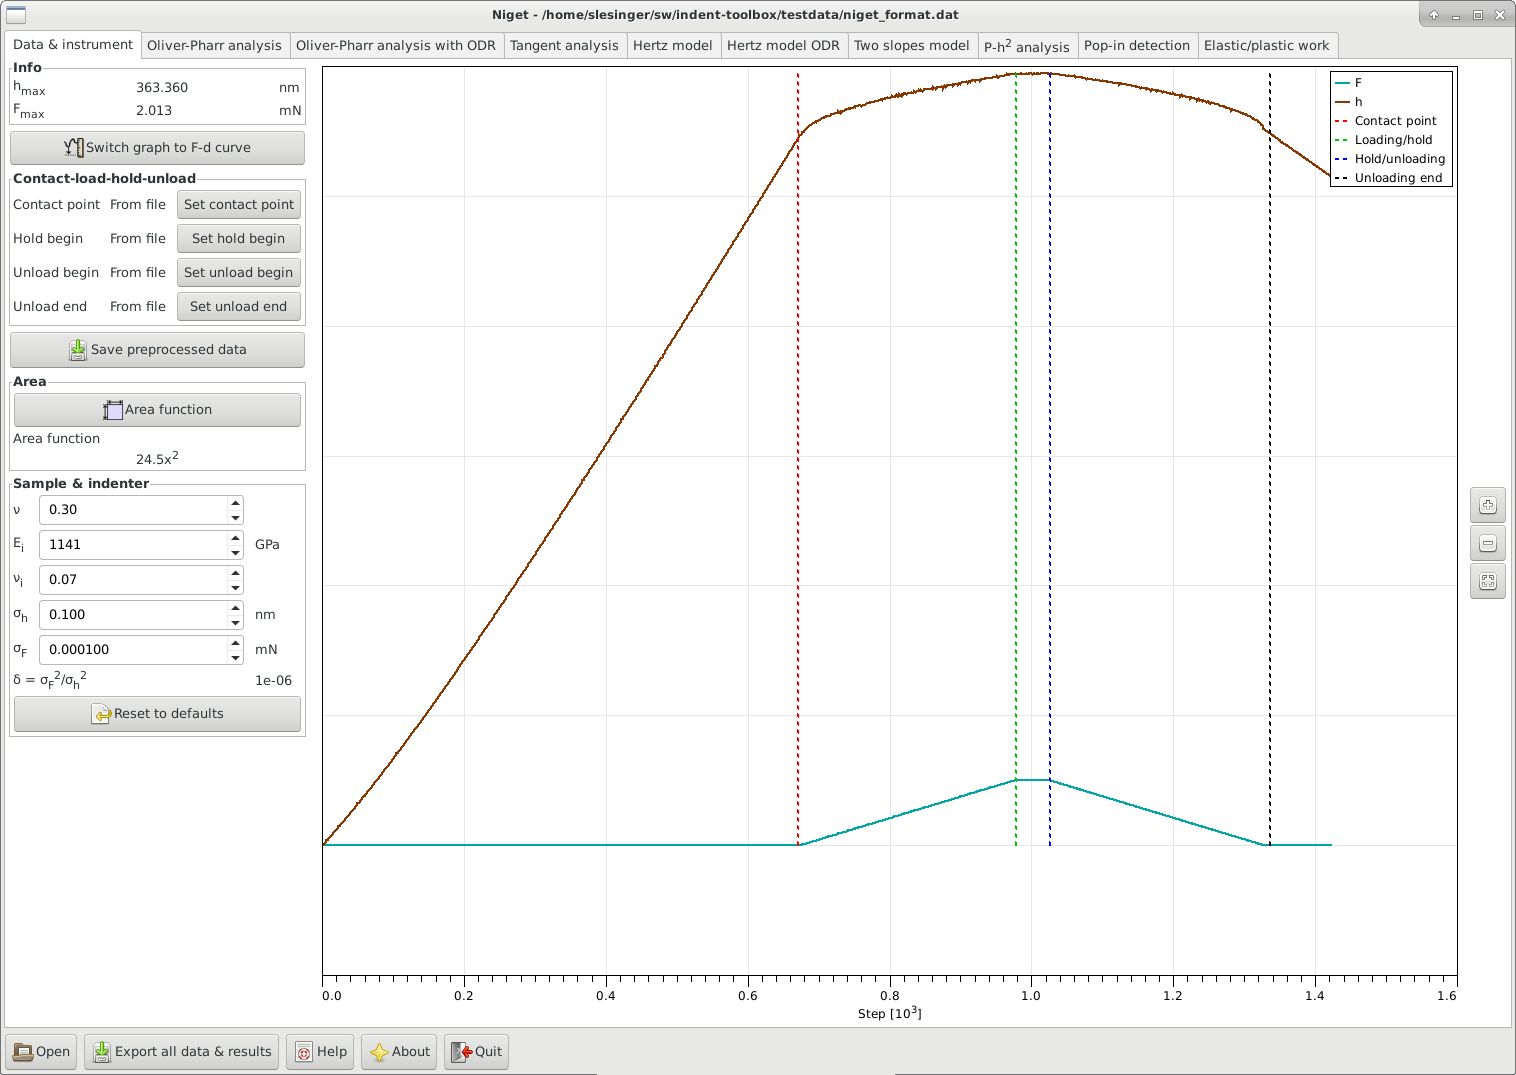
\includegraphics[width=\textwidth]{images/screen-fdtime}
  \caption{Manual definition of points in force-distance in time view}
\end{figure}

\subsection{Window}
The window consists of the following:
\begin{itemize}
 \item \emph{Info} displays the maximum depth and force during the indentation determined as in section \ref{contact_max}. 
 \item \emph{Switch graph to \dots} switches between two display modes: force as a function of depth (F-d) and force and depth as functions of the (pseudo)time (F,d-t). The index of the data point is used instead of the real time, which is not read from the file.
 In the second case, both curves are displayed dimensionless, and scaled just to provide good visual resolution.
 \item \emph{Contact-load-hold-unload} Allows to manually split the data into the loading, hold and unloading parts:
 \begin{itemize}
 \item[-] Contact point: determines the beginning of the loading curve. The depth and force at this point $h_c$ and $F_c$ are subtracted from the loading-unloading curves.
 \item[-] Hold begin
 \item[-] Unload begin 
 \item[-] Unload end: define the end of the unloading part. By default, the data are truncated at zero depth.
\end{itemize}
  Whether the point was set automatically or manually is shown. Note, that if the division of the data into the different parts is changed, all analysis results are deleted!
 \item \emph{Save preprocessed data} saves the data including the selected split of the data in the native format Niget. 
 \item \emph{Area}
 \begin{itemize}
 \item[-] Area function button: opens a separate dialog for the definition of the area function, see \ref{area}
 \item[-] displays the area function used currently.
 \end{itemize}
  \item \emph{Sample \& indenter}
    The parameters here are Poisson's value of the sample, Young's modulus of the indenter, Poisson's value of the indenter and the noise of the displacement and load sensors. The default values are 0.3, 1141~GPa, and 0.07. 
    The first is a reasonable estimate of the often unknown Poisson's value for many materials, the other two values are the literature values for diamond which is a common indenter tip material. 
    The noise of the sensors is used for the fitting procedures and for the uncertainty analysis.
    These values are saved in settings and can be reset to their default values.
\item \emph{Graph}  displays the indentation curve.  Stepwise zooming/unzooming can be performed by selecting a range with the mouse and pressing the \emph{Zoom}/ \emph{Unzoom} buttons. The graph is restored to its original size by the \emph{Restore} button.
The zooming procedure is independent in the two regimes (F-d vs. F,d-t).
\end{itemize}

\subsection{Maximum depth and force} \label{contact_max}
The maximum force $\Fmax$ is the maximum force value found in the unloading data. The maximum depth $\hmax$ is the corresponding depth, NOT the maximum depth value!

\subsection{Area function} \label{area}
The area function can be given either in form of a polynomial of the form
\begin{equation} \label{eq:Aphc}
A(h) = c_2 h^2 + c_1 h + c_{1/2} h^{1/2} + c_{1/4} h^{1/4} + c_{1/8} h^{1/8} + c_{1/16} h^{1/16},
\end{equation}
or a raw data file can be loaded, which will be (linearly) interpolated in subsequent calculations. The format of the area data file MUST be two columns: first column depth in nm, second column area in nm$^2$.\\ 
The area function is shown for user information. A warning is issued if a raw data file is used and any of the methods extrapolates the area. 
The coefficients of a polynomial area function are saved in the settings file. 

For specific formats, the coefficients can also be loaded directly from a file. 
Currently, this should work for an \verb|.ara| file (as exported from a Hysitron instrument) or for an \verb|.ind| file (as exported from a UNHT Anton Paar instrument). 
This is under testing and may not work correctly for other versions. 

\begin{figure}[h]
  \centering
  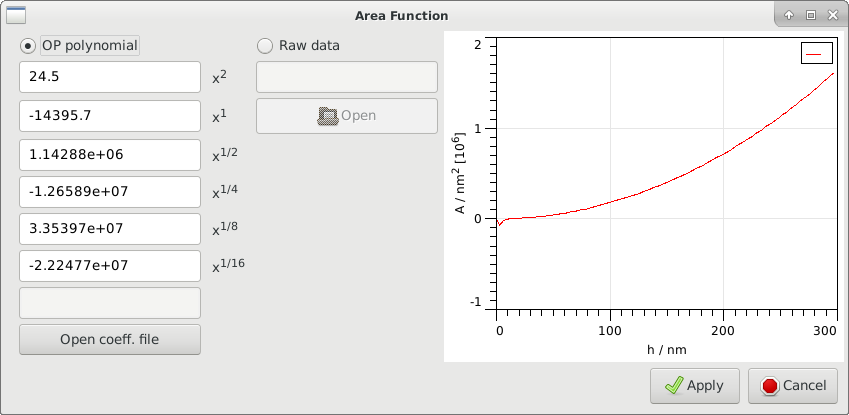
\includegraphics[width=.6\textwidth]{images/screen-area}
  \caption{Area function dialog}
\end{figure}
